\documentclass[10pt,twocolumn]{article}

% formatting
\paperwidth=8.5in
\paperheight=11in
\setlength{\columnsep}{0.25in}
\usepackage{leading}
\usepackage[margin=0.5in]{geometry}

\usepackage{times}
\usepackage{listings, textcomp}
\usepackage[T1]{fontenc}

\usepackage{amsmath}
\usepackage{booktabs}
\usepackage{graphicx}
\usepackage{enumitem}
\usepackage[hidelinks]{hyperref}
\hypersetup{breaklinks=true}
\Urlmuskip=0mu plus 2mu
\usepackage{subcaption}
\usepackage{xcolor}
\usepackage{flushend}

\newcommand{\remark}[1]{{\color{red}[#1]}}

\makeatletter
\setlength{\@fptop}{0pt}
\makeatother

\begin{document}

\leading{11pt}

\title{\bf Contextual Code Completion Using Machine Learning}
\author{Subhasis Das, Chinmayee Shah\\
        \{subhasis,~chshah\}@stanford.edu\\
        Mentor: Junjie Qin}

\date{}
\maketitle
\thispagestyle{empty}

\begin{abstract}
Large projects such as kernels, drivers and libraries follow a code
style, and have recurring patterns. In this project, we explore learning based
code recommendation, to use the project context and give meaningful
suggestions.
Using word vectors to model code tokens, and neural network based learning
techniques, we are able to capture interesting patterns, and predict code that
that cannot be predicted by a simple grammar and syntax based approach as in
conventional IDEs.
We achieve a total prediction accuracy of 56.0\% on Linux
kernel, a C project, and 40.6\% on Twisted, a Python
networking library.

\end{abstract}
\section{Introduction}
\label{sec:intro}

\noindent
Code IDEs such as Eclipse and Microsoft Visual Studio make the task of writing
code in new languages easier by auto-completing key words and phrases.
For example, when writing code in C++, an IDE may automatically close an
opening parenthesis, and suggest else immediately following an if block.
Such code completion has several problems:
\begin{enumerate}[topsep=0pt,itemsep=-1ex,partopsep=1ex,parsep=1ex]
  \item Grammar based code completion requires writing down an exhaustive set
    of rules. This is tedious and repetitive when done for every new language.
  \item Predictions do not consider the category of code. For instance, driver
    codes and math libraries may exhibit different patterns.
  \item Predictions do not consider context such as header file, class
    definition, function definition, tabs and spaces, opening and closing
    braces on the same line.
  \item Recommendations are often ordered lexicographically, which means some
    of the top recommendations may not be useful.
\end{enumerate}

\noindent
This report explores a learning based approach to code completion. Instead of
writing grammar based rules, we use machine learning to learn structure and
patterns in code. We can then not only automate code predictors for different
languages, but also specialize them for different kinds of projects such as
drivers and libraries. We can also consider the enclosing context and rank
predictions.
%Section~\ref{sec:model} describes our model for the problem of code completion.
%It also gives a brief overview of a word vector based approach to modeling
%tokens in code, and techniques we use to work with a limited volcabulary of
%words.
%Section~\ref{sec:memoryless} presents memoryless techniques for predicting
%based on only a small window of preceeding tokens. While these techniques use
%less contextual information, we can still train them for different languages
%and projects.
%Section~\ref{sec:window} presents results about the influence of different
%tokens on the output.
%Section~\ref{sec:conclusions} presents conclusions about the techniques that we
%have explored so far, and proposes stateful techniques for using more immediate
%context such as file based context to improve predictions.

%\vspace{-5pt}
\section{Related Work}
\label{sec:related}

We use natural language techniques for predicting code.
In this section, we review some literature on language models and
neural network based language models.

\subsection{Traditional Language Models}
Statistical models of languages have been used extensively in various natural
language processing tasks. One of the simplest such models proposed is the
$n$-gram model, where the frequencies of consecutive $n$ tokens are used to
predict the probability of occurence of a sequence of tokens. The frequencies of
such $n$-grams are obtained from a corpus, and are smoothed by various
algorithms such as Kneser-Ney smoothing~\cite{ref:kneser-ney} to account for
sparsity of $n$-grams. Such models can be easily extended to code completion,
by modeling each token as a word and doing $n$-gram analysis over a
codebase. However, such models do not capture
the high fraction of unknown tokens from variable and function names very well.
%used for code completion considering the high fraction of {\tt UNKNOWN} tokens
%in codes. For example, even in a simple case such as {\tt for(int SOMEVAR = 0;
%SOMEVAR < EXPRESSION; SOMEVAR++)}, the token {\tt SOMEVAR} can be arbitrary, and
%{\tt EXPRESSION} can consist of multiple tokens. Also, it has been shown that
%neural network based language models far outperform such traditional language
%models. Hence, in our work, we only consider neural network based language
%models.

\subsection{Word Vector Embeddings and Neural Network Language Models (NNLM)}
In their seminal work, Bengio et al.~\cite{ref:embedding} first propose a
vector embedding space for words for constructing a language model,
that significantly outperforms traditional $n$-gram based
approaches. Their proposal maps each word to a vector and expresses the
probability of a token as the result of a multi-layer neural network on the
vectors of a limited window of neighboring words. T. Mikolov
et al.~ \cite{ref:regularities} show that such models can capture word-pair relationships
(such as ``{\em king} is to {\em queen} as {\em man} is to {\em woman}'') in
the form of vector operations (i.e., $v_{\text king} -
v_{\text queen} = v_{\text man} - v_{\text woman}$). To distinguish such models
from {\it recurrent} models, we
call them {\it feed-forward} neural network language models.
We use the same concept in our token-embedding. We found singificant clustering
of similar tokens, such as {\tt uint8\_t} and {\tt uint16\_t}, but were unable
to fund vector relationships.
%We use the same concept in our token-embeddings, where we attempt to predict
%probabilities of the next token depending on the token-vectors of a fixed window
%of prior tokens.
%We were able to observe significant clustering in the word
%vectors of similar tokens (e.g., vectors of {\tt uint8\_t} and {\tt uint16\_t}
%are very similar). However, we were {\it unable} to find vector relationships
%between tokens such as those discussed above.

Later, such feed-forward NNLMs have been extended by Mikolov et
al.~\cite{ref:mikolov:wvec} where they propose the continuous
bag-of-words (CBOW), and the skip-gram. In CBOW, the probability of a token is
obtained from the average of vectors of the neighboring tokens, whereas in
skip-gram model the probabilities of the neighboring tokens is obtained from the
vector of a single token. The main advantage of such models is their
simplicity, which enables them to train
% relative to a multi-layer feed-forward network, which enables them to be trained
faster on billion-word corpuses. However, in our case, the size of data was not
so huge, and we could train even a 4-layer model in 3 days.

\subsection{RNN Language Models}
\label{sec:rel:rnnlm}
A significant drawback of feed-forward neural network based language models is
their inability to consider dependencies longer than the window size. To fix
this shortcoming, Mikolov et al. proposed a recurrent neural network based
language model~\cite{ref:rnnlm}, which associates a cell with a hidden state
at each position, and updates the state with each token. Subsequently, more
advanced memory cells such as LSTM~\cite{ref:lstm} and GRU~\cite{ref:gru} have
been used for language modeling tasks. More sophsticated models such as
tree-based LSTMs ~\cite{ref:treelstm} have also
been proposed. We experimented with using GRUs in our setup, but surprisingly
did not find them to be competitive with feed-forward networks.

\subsection{Attention Based Models}
\label{sec:attn}
Recently, neural network models with {\it attention}, i.e., models that weigh
different parts of the input differently have received a lot of attention (pun
intended) in areas such as image captioning~\cite{ref:showattendtell} and
language translation~\cite{ref:nmt,ref:nmt2}. In such models, the actual task of
prediction is separated into two parts: the attention mechanism which
``selects'' the part of input that is important, and the actual prediction
mechanism which predicts the output given the weighted input. We found an
attention based feed-forward model to be the best performing model among the
ones we considered.

\subsection{Code Completion}
\label{sec:code-completion}
Frequency, association and matching neighbor based
approaches~\cite{ref:learningexamples} are used to improve predictions of IDEs such
as Eclipse.
Our learning approach, on the other hand, attempts to automatically
learn such rules and patterns.

%\vspace{-5pt}
\section{Dataset and Features}
\label{sec:dataset}

We use two different projects, Linux source~\cite{ref:linuxcode}, a C project,
and Twisted~\cite{ref:twistedcode}, a Python networking library, to train and
test our methods. In each case, we use half of all files for training, and the
remaining half for testing.
Given a sequence of tokens in an incomplete piece of code,
we predict the next token.
We pick these incomplete code pieces randomly from the complete codes in the
training set.
Tokens in these incomplete codes constitute the features, and the next token
occuring in the actual complete code is the "truth".
The next section describes how we model these tokens.

%\vspace{-5pt}
\section{Modeling Tokens}
\label{sec:model}

\noindent
One of our objectives of learning based code prediction is to do away with the
tedious process of building grammar based rules for different languages.
We treat codes in the training set in a language agnostic way. The first step
is to build a dictionary of tokens or words that can occur in the code, that we
can take as input to predict the next token. We build this dictionary by
reading all code, and treating each consecutive set of alphanumeric characters
and (\_), or each consecutive set of special characters other than alphanumeric,
(\_), space and newline as one token.  Thus, for example, the code {\tt for
(my\_var = 0; my\_var < foo; my\_var++) \{} will be tokenized into eleven
tokens: {\tt for}, {\tt my\_var}, {\tt =}, {\tt 0}, {\tt ;}, {\tt my\_var}, {\tt
<}, {\tt foo}, {\tt;}, {\tt my\_var}, {\tt++) \{}.  Given a sequence of tokens, we
then want to predict the next token. Note that these tokens do not correspond
exactly to language level tokens, e.g., {\tt++) \{} is a single token despite
containing three different language level tokens {\tt++}, {\tt)}, and
{\tt\{}.

The dictionary of tokens constructed as above is not complete, since new code
may contain new tokens that are not present in the training data. Moreover,
many of the tokens in the training data may be specific to a few files and may
never occur again. To address these issues, we divide the tokens into two
categories:

a) {\it Key tokens}: A subset of $K$ most frequent tokens are categorized as
{\it key tokens}. Not surprisingly, many of
these frequent tokens are keywords for the language the project is written in,
or words that tend to occur often in that
particular project.
For example, some of the frequent tokens in Linux kernel are:
\texttt{struct}, \texttt{;}, and \texttt{dev}, out of which the first and second
are keywords in C, and the third is a token frequently used to denote device
objects in Linux. Note that while several language keywords do end up being part
of the set of key tokens, we {\it do not} manually curate the list of key tokens
to ensure that they contain only language specific keywords.

b) {\it Positional Tokens}: While key tokens occurrences constitute a major
fraction of all token occurrences ($\approx$ 60\% with 2000 key tokens),
the remainder of tokens are rarely
seen (such as names of variables, macros etc.). However, we would like our
learning algorithm to autocomplete new variable names, once they occur in a
file. For
example, given many examples of the form {\tt for (int TOKEN = 0; TOKEN < n;
TOKEN++)} (all with different values of {\tt TOKEN}), our algorithm should be
able to autocomplete {\tt for (int myIterName = 0;} with {\tt myIterName}. This
capability can not be achieved by merely trying to autocomplete between a set of
pre-defined key tokens. Hence, we also define {\it positional tokens} as follows.

Given a sequence of tokens --- an incomplete piece of code, we replace each
token which is not a key token by a string of the form {\tt
POS\_TOK\_ii}, where {\tt ii} is the {\it position} of that token
within that sequence. A non-keyword token which is repeated multiple times in a
sequence is assigned the index corresponding to its first appearance. For
example, given the sequence of tokens {\tt[for, int, myVarName, =, 0, ;,
myVarName, <, n, ;, myVarName, ++]}, where {\tt myVarName} is not a key token,
we construct the new sequence {\tt[for, int, POS\_TOK\_2, =, 0, ;, POS\_TOK\_2,
<, n, ;, POS\_TOK\_2, ++]}. In case the token to be predicted is not a key token
but has appeared in the window, it is also replaced by the corresponding
positional token string. If the target has not appeared before in the window, it
is assumed to be a special token {\tt UNKNOWN}. However, as we describe in
Section~\ref{sec:methods}, we ignore such windows since in many such
cases the token is actually a hereto unseen token.

Such an encoding is advantageous since now the set of prediction targets to
choose from is simply the union of the key tokens and the positional token
strings (of the form {\tt POS\_TOKEN\_ii}). In case of a fixed window size of
$W$ and a fixed number of key tokens $K$, it can be seen that the total number
of prediction targets is $K+W+1$ ($K$ key tokens, $W$ positional tokens, and 1
unknown token), i.e., a {\it constant}. This immediately opens up the
possibility of applying simple models such as logistic/neural network based
classifiers.

%\vspace{-5pt}
\section{Methods}
\label{sec:methods}

\noindent
In this model, we simply take the set of $K+W$ positional and key tokens, and
the set of $K+W+1$ output tokens, and fit a model similar to word
vectors~\cite{ref:mikolov:wvec}. The details of the model are described below.

We first assign a $D$ dimensional vector to each one of $K+W$ different key
tokens and positional tokens. We denote such token-vectors by $v_i$, where $1
\leq i \leq K+W$. Next, given a fixed size window of tokens $[t_1, t_2, \ldots,
t_W]$, we compute a score for each possible output $j$, $s_j$ as a function of
the token-vectors of the tokens in the window, i.e.,
\[
s_j = f_j\left(v_{t_1}, v_{t_2}, \ldots v_{t_W}\right)
\]
The final loss function for this particular example is given by 
\[
L = \log\left(\frac{e^{s_{t_o}}}{\sum_j{e^{s_j}}}\right)
\]
where $t_o$ is the output token. This is the cross-entropy loss
between softmax based probabilities for each output and the actual observed
output. According to the actual form of the function $f_j$, we get different
models. A few of these models are described below.

For each model, we use {\sc AdaGrad} optimizer to minimize the total loss
function with respect to the parameters of that model. {\sc AdaGrad} was chosen
because it gave the best performance in our case among other alternatives such
as vanilla SGD and momentum based SGD.

\subsection{Fixed Window Weight Model}
In the spirit of continuous bag-of-word (CBOW) model~\cite{ref:mikolov:wvec}, in
this model we assume that a token at position $i$ has a ``weight'' of $w_i$, and
combine the token-vectors of the window according to these weights. The final
score is assumed to be a linear function of this weighted token-vectors. Thus,
the overall model is
\begin{align}
u &= \sum_{i=1}^{W}{w_i v_{t_i}}\\
s_j &= p_j^Tu\\
L &= \log\left(\frac{e^{s_{t_o}}}{\sum_j{e^{s_j}}}\right)
\end{align}
The parameters in this model are the weights $w_i$, the word vectors $v_i$, and
the ``prediction'' vectors $p_j$. The gradients of the loss w.r.t. the
parameters are obtained by backpropagation, the details of which are omitted
here for space.

\subsection{Matrix Vector Model}
In this case, we do not introduce any averaging as in the case of CBOW, but
instead simply concatenate the token-vectors to create a larger vector which is
then used to create the scores. Formally, the model is
\begin{align}
u &= [v_{t_1}; v_{t_2}; v_{t_3}; \ldots; v_{t_W}]\\
s_j &= p_j^Tu\\
L &= \log\left(\frac{e^{s_{t_o}}}{\sum_j{e^{s_j}}}\right)
\end{align}
Note that since here $u$ is $DW$ dimensional instead of being $D$ dimensional as
in the case of Fixed Window Weight Model. Thus, the prediction vectors $p_j$ are
much higher dimensional as well, which means this model has a higher number
of parameters as compared to Fixed Window Weight Model.

\subsection{Feed-Forward Neural Network Model}
\label{sec:nnlm}
This case differs from the Matrix Vector Model by addition of one or more
non-linear transformations between the concatenated token-vectors and the final
scores. We denote a specific instance of this model by NL-$k$, where $k$ is the
number of non-linearity layers it contains. Thus, for example, NL-$0$ is
equivalent to the Matrix-Vector model described above, while for NL-$3$ the
probabilities are obtained as:
\begin{align}
u &= [v_{t_1}; v_{t_2}; v_{t_3}; \ldots; v_{t_W}]\\
z_1 &= \text{relu}(Q_1u)\\
z_2 &= \text{relu}(Q_2z_1)\\
z_3 &= \text{relu}(Q_3z_2)\\
s_j &= p_j^Tz_3\\
L &= \log\left(\frac{e^{s_{t_o}}}{\sum_j{e^{s_j}}}\right)
\end{align}
Here $\text{relu}(.)$ is the rectified linear unit, i.e., $\text{relu}(x) = x$
if $x \geq 0$, and $0$ otherwise. In this work, we specifically experimented
with NL-$0$, NL-$1$, NL-$2$, and NL-$3$.

\subsection{Feed-Forward Model with Soft Attention}
\label{sec:annlm}
Motivated by the recent successes of attention based models, we explore an
attention mechanism for our problem as well. We experiment with a
``soft''-attention model, i.e., a weight $a_i$ between 0 and 1 is assigned to
each position $i$. The attentions are assumed to be the result of a sigmoid
function on a linear combination of the concatenated word-vectors. Subsequently,
the word vector for the $i^{th}$ token is weighted by $a_i$, and the
aforementioned NL-$k$ model is applied on the concatenation of these weighted
word vectors instead. Thus, for example, an attention based NL-$3$ model takes
the form of:
\begin{align}
u &= [v_{t_1}; v_{t_2}; v_{t_3}; \ldots; v_{t_W}]\\
a &= \sigma(Au)\\
z &= [a_1v_{t_1}; a_2v_{t_2}; a_3v_{t_3}; \ldots; a_Wv_{t_W}]\\
s_j &= \text{NL-}3(z ; Q_1, Q_2, Q_3, p_j)\\
L &= \log\left(\frac{e^{s_{t_o}}}{\sum_j{e^{s_j}}}\right)
\end{align}
Here NL-$3(x ; Q_1, Q_2, Q_3, p_j)$ is the function going from $u$ to $s_j$ in
the case of a NL-$3$ model, described in Section~\ref{sec:nnlm}.

\subsection{GRU based Recurrent Model}
\label{sec:rnnlm}
Recurrent neural network models based on cells like LSTM~\cite{ref:lstm} and
GRU~\cite{ref:gru} have recently been shown to achieve state-of-the-art
performance in language models. Inspired by these results, we also attempted to
use a GRU based recurrent model for our prediction task. Specifically, our model
was the following:
\begin{align}
[g_1; g_2; g_3; \ldots; g_{W}] &= \text{GRU}([v_{t_1}; v_{t_2}; v_{t_3}; \ldots;
v_{t_W}])\\
s_j &= p_j^T[g]\\
L &= \log\left(\frac{e^{s_{t_o}}}{\sum_j{e^{s_j}}}\right)
\end{align}
Here, $g_i$ is the output of the $i^{th}$ GRU cell, and we have a dense layer
after that to get the scores for each output token. As we did not achieve
competitive performance with this model as compared to NL-$1$, we did not
experiment further with deeper GRU models.

%\vspace{-5pt}
\section{Experiments and Results}
\label{sec:results}

In this section, we evaluate the methods outlined in Section~\ref{sec:methods},
on Linux kernel and Twisted library. We first present the accuracy of
predictions on the test set, and then present some interesting predictions that
come out from recurring patterns. We implemented the matrix vector model in
Python, and the feed-forward and recurrent models in Keras~\cite{ref:keras}.
Our code is available on github~\cite{ref:codecompletion}.

\subsection{Accuracy}
\label{sec:accuracy}

\begin{table}[h]
  \centering
%  \small {
  \begin{tabular}{l l l r r r r r}
    \hline
    Method & Known & Abs & Top 3 & Key & Pos \\
    Win, \#Keys & acc. & acc. & acc.  & acc. & acc. \\
    \hline
    NL-3, 40, 2000 & 64.4 & 53.4 & 81.7 & 78.0 & 43.7\\
    NL-4, 64, 2000 & 63.2 & 50.6 & 82.0 & 72.8 & 41.8\\
    Attn, 40, 1000 & 67.5 & 56.0 & 83.6 & 79.9 & 48.4\\
    BestKW-RandPos & 49.8 & 41.3 & -- & 79.9 & 7.0\\
    \hline
  \end{tabular}
%  }
  \caption{Test accuracy (\%) of predictions for Linux project}
  \label{tab:linux}
\end{table}

\begin{table}[h]
  \centering
%  \normal {
  \begin{tabular}{l l l r r r r r}
    \hline
    Method & Known & Abs & Top 3 & Key & Pos \\
    Win, \#Keys & acc. & acc. & acc.  & acc. & acc. \\
    \hline
    NL-3, 40, 500 & 46.3 & 39.2 & 64.8 & 64.1 & 14.2\\
    NL-4, 40, 500 & 44.8 & 37.7 & 62.2 & 63.9 & 10.8\\
    Attn, 40, 500 & 47.9 & 40.6 & 66.5 & 64.6 & 17.6\\
    GRU, 40, 500 & 41.6 & 35.2 & 59.1 & 64.4 & 4.9\\
    BestKW-RandPos & 43.6 & 37.5 & -- & 64.4 & 5.5\\
    \hline
  \end{tabular}
%  }
  \caption{Test accuracy (\%) of predictions for Twisted project}
  \label{tab:twisted}
\end{table}

\noindent
Table~\ref{tab:linux} shows results for Linux source, a C project, and
Table~\ref{tab:twisted} for Twisted, a Python networking library. As mentioned
in Section~\ref{sec:dataset}, we use half the files for training and half for
testing.
Column 1
lists the learning method, window size and number of key words.
NL-3 is a feed forward model with 3 non-linearity layers, and NL-4 is a feed
forward model with 4 non-linearity layers. Attn. computes a weighing
parameter for each input token in the window, and uses 3 non-linearity layers.
GRU is a recurrent model. We do not report numbers for GRU in the Linux codebase
since it gave poor results in the smaller Twisted codebase.
Additionally, we report numbers for a fictional random
predictor that achieves the accuracy of the best predictor in case of keywords,
but in case of a non-keyword token predicts one randomly from the non-keyword
tokens in the window, to show the significance of positional tokens.
We name this BestKW-RandPos.

Known acc. is the
accuracy for predictions for the cases where the next token is a key token, or
a positional token from the window being considered. Abs acc. is the accuracy
for predictions for all cases, including cases where the next token is
neither a key word nor a seen positional token. These are often new function
names or variable names, or variables outside of our window. Top 3 is the
percentage of cases where the next token is within top 3 predictions, ignoring
the unknown cases (unseen variable and function names).
We report this number, because generally, we are interested in the top few
suggestions as opposed to the top suggestion with a code recommendation system.
Key acc. is the
accuracy with which we predict key tokens correctly, given the next token is a
key token,
and pos. acc. is the accuracy with which we predict positional tokens
correctly, given the next token is a positional token.
These give us insight into how well our methods predict tokens that are not key
tokens.

We found that attention gives the best results among all the methods we tried.
This makes sense because it is also the most general of all models --- it
directly connects all inputs to the output, (unlike GRU where computed states
are chained), and it has an additional attention parameter, that is just a
constant in the simple feed-forward case. We also found that the feed forward
model with 4 non-linearity layers tends to overfit the training data, giving a slightly
lower accuracy on test data. Increasing the word vector dimensions also tends
to result in overfitting. Though regularization can help with overfitting, we
found that reducing vector dimensions and number of layers was also sufficient
to reduce high variance from overfitting.

The accuracy of predicting non-key words, that is, positional tokens is quite
high for Linux kernel, a C project, indicating there is a lot of redundancy/
recurring patterns. The positional token accuracy is lower for Python.
We think this is because Python is a dynamically typed, high level
language with less redundancy, and more terse syntax.
However, in both cases, the top 3 prediction
accuracy is still much higher than a random predictor, indicating that the
model does extract some patterns out of the code.

A plot of the word vectors reveals a significant clustering of similar
words --- {\texttt {uint8\_t}} and {\texttt {uint16\_t}}, different locking and
unlocking calls, and integers. We have omitted these plots from the report for
space. Unlike natural language texts, however,
we did not observe any significant vector relationships between different
tokens.

\subsection{Examples}
\label{sec:examples}
Another experiment we ran was to evaluate the accuracy of the classifier in a
setting where, if the correct token is not within the top few predictions, the
user types in one or more characters to ``home in'' on the correct prediction.
Figure~\ref{fig:codeexample} shows the results for this experiment. In this
experiment, a character is colored in green if the token is correctly predicted
(i.e., top prediction) before that character is typed. It is colored in yellow
if the token is among the top 5 before typing that character, and colored in red
if the token is not among the top 5. So, for example, in the first line in the
token
{\tt struct}, the character {\tt s} is in yellow since before typing {\tt s}, the
token {\tt struct} was among the top 5. After typing {\tt s}, the top prediction
was {\tt struct}, and thus the characters {\tt truct} are all in green. We
can see that, for example, entire sequences of code such as {\tt \{
PCI\_VDEVICE(SUNDANCE, } are predicted correctly without typing anything.
\begin{figure}[h]
  \centering
  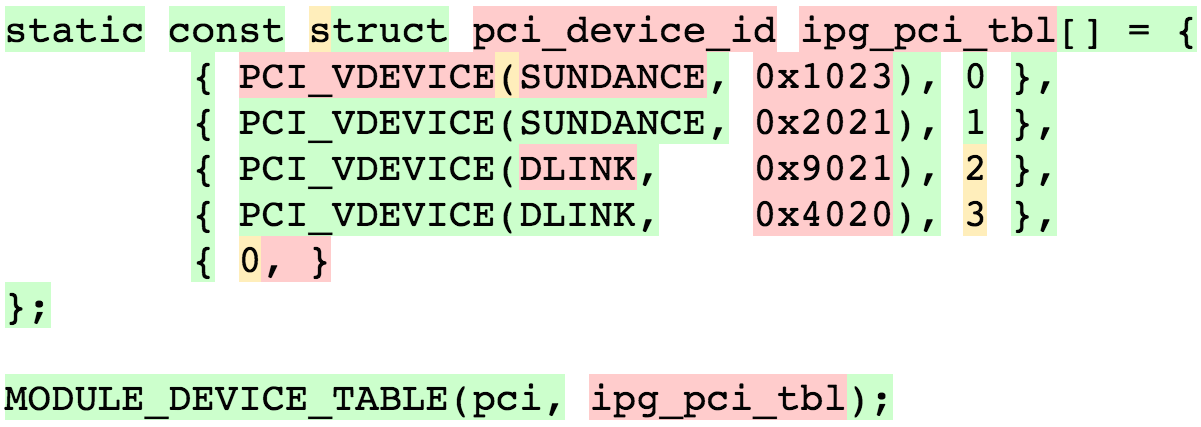
\includegraphics[width=\linewidth]{figs/example3.png}
  \caption{Code example with per-character predictions}
  \label{fig:codeexample}
\end{figure}

\subsubsection{Importance of Positional Tokens}
From Figure~\ref{fig:codeexample} we can also see the importance of positional
tokens. The tokens {\tt PCI\_VDEVICE} and {\tt SUNDANCE} are both not keywords
(i.e., not frequently observed in the codebase), and yet were predicted
correctly by our method the second time they were used (in line 3). If we chose
to ignore such tokens instead, we would not have been able to predict such
tokens correctly in a majority of cases.

\subsubsection{Learning Frequently Occurring Patterns}
We also found several interesting patterns that are predicted correctly by our
system. An example of such a pattern is given in
Figures~\ref{fig:conditional1}~\&~\ref{fig:conditional2}. In these figures, each
character is color coded as before, and some additional information is also
shown. The top 5 predictions at the position of interest (shown in red border),
are shown in a blue box. Also, the value of attention for each token in the
prediction window are shown color coded in sky-blue, where deeper blue is
indicative of more attention (for reference, the first {\tt if} tokens in both
of these two cases have an attention value of $\approx$ 1).

\begin{figure}
  \centering
\begin{subfigure}{\linewidth}
  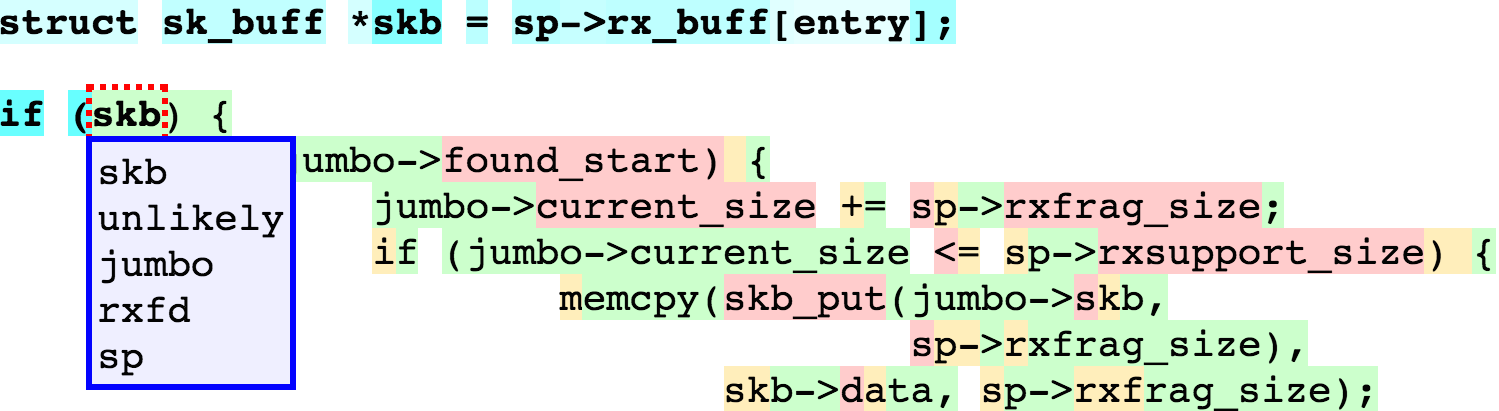
\includegraphics[width=\linewidth]{figs/example8.png}
  \caption{Example 1}
  \label{fig:conditional1}
\end{subfigure}
\begin{subfigure}{\linewidth}
  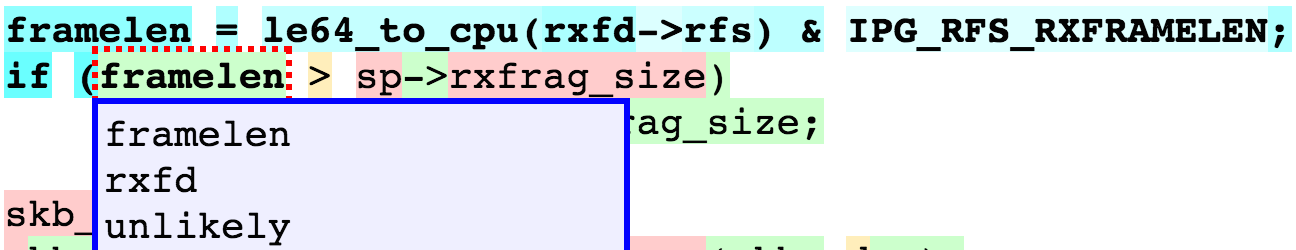
\includegraphics[width=\linewidth]{figs/example9.png}
  \caption{Example 2}
  \label{fig:conditional2}
\end{subfigure}
  \caption{Definition before {\tt if} pattern}
  \label{fig:ifpattern}
\end{figure}

Here, a variable is assigned to right before an {\tt if} statement, and the
prediction is that the variable will be immediately used inside the {\tt if}
condition. This is a common pattern in Linux code, where if the condition inside
{\tt if} is too long, it is broken up into an assignment and a subsequent
conditional.

Also, in the figure the top 5 predictions for each case is given in the blue
box. We can see that {\tt unlikely} is a common prediction, since {\tt if
(unlikely(condition))} is a common pattern in Linux code to check for unlikely
edge cases such as error conditions.

We can also see that the attention of the models is relatively high at the
correct predictions ({\tt skb} and {\tt framelen} in the first and second cases
respectively). This shows that even a single layer model can be expected to
fairly reliably predict the next token (since the attention is derived from a
single non-linear layer).

A few more interesting examples are shown in Figure~\ref{fig:moreexamples}. A
description of why each of the cases are interesting are given in the captions.

\begin{figure}[t!]
  \centering
\begin{subfigure}{\linewidth}
  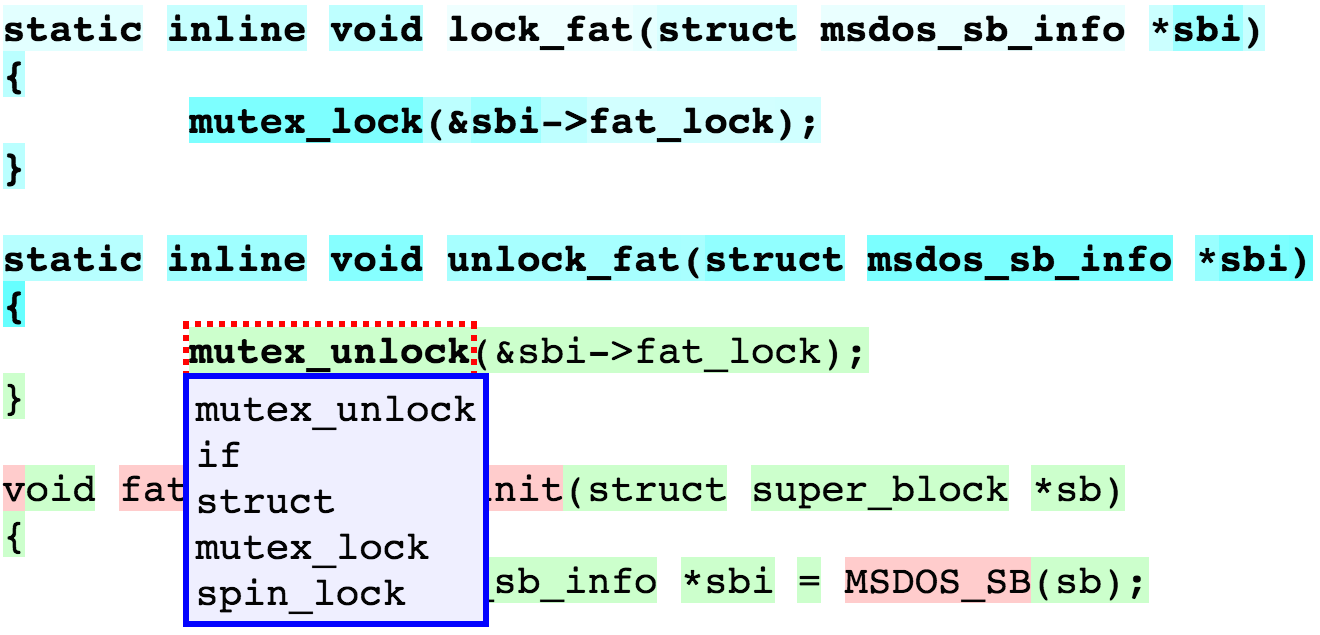
\includegraphics[width=\linewidth]{figs/example10.png}
  \caption{{\tt mutex\_lock} and {\tt mutex\_unlock} pair on same lock variable}
  \label{fig:lockunlock}
\end{subfigure}
\begin{subfigure}{\linewidth}
  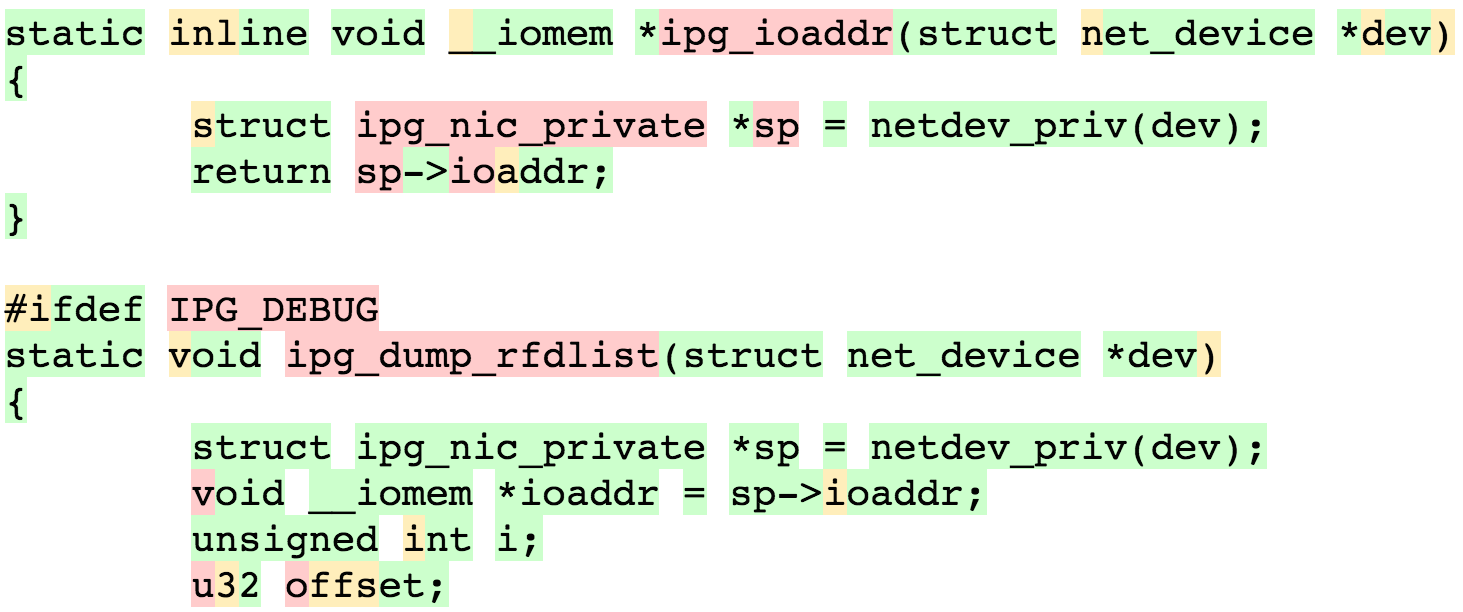
\includegraphics[width=\linewidth]{figs/example4.png}
  \caption{Duplicate code after function definition predicted correctly}
  \label{fig:duplicate}
\end{subfigure}
\begin{subfigure}{\linewidth}
  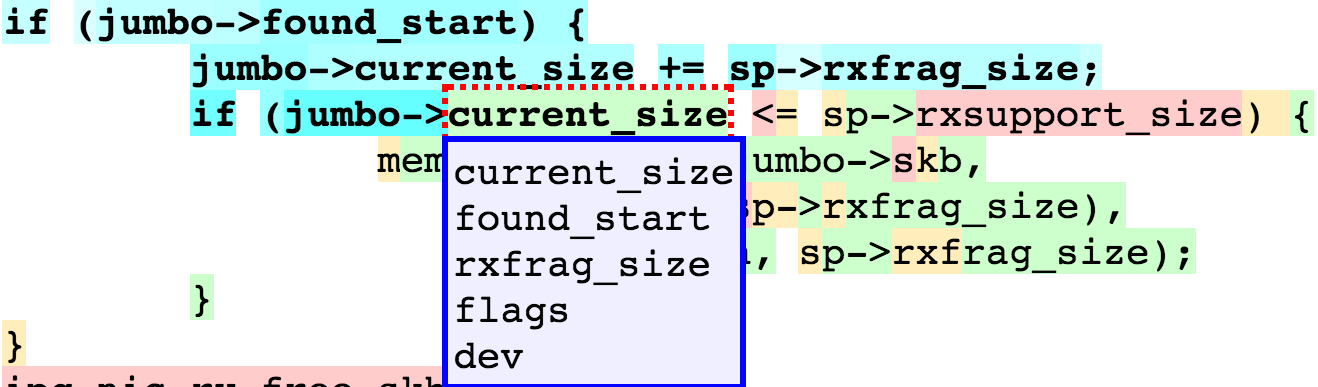
\includegraphics[width=\linewidth]{figs/example7.png}
  \caption{Member variables predicted correctly}
  \label{fig:memvar}
\end{subfigure}
\begin{subfigure}{\linewidth}
  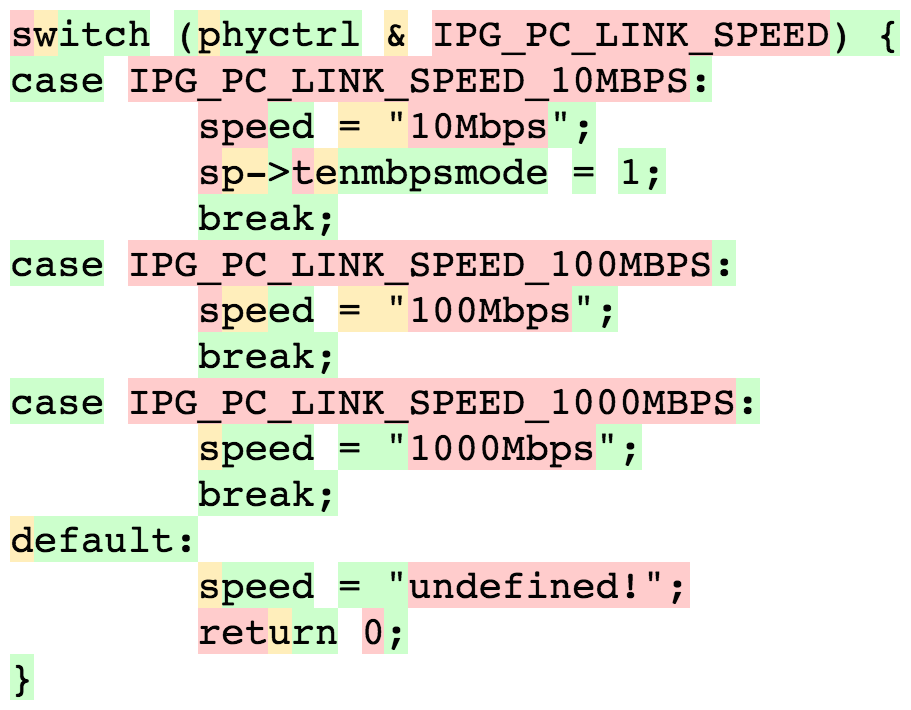
\includegraphics[width=0.6\linewidth]{figs/example1.png}
  \caption{{\tt case} token predicted correctly after each {\tt break;}}
  \label{fig:breakcase}
\end{subfigure}
  \caption{Interesting code patterns predicted correctly}
  \label{fig:moreexamples}
\end{figure}

%\vspace{-5pt}
\section{Conclusions and Future Work}
\label{sec:conclusions}

\noindent
Among the methods we tried so far, chaining two matrix-vector models with a
relu nonlinearity performs the best.
This is also the most general of all models we tried, so
the higher accuracy is not surprising. Given the results for correlation between
input and target tokens, we would like to experiment with larger windows
where we exclude odd tokens.

The word vector algorithms we tried so far do not capture file specific
patterns. Non-key tokens that are local to the file, and outside the window are
ignored. We want to try out a recurrent neural network (RNN)
approach~\cite{rnn} or a long short-term memory (LSTM) approach~\cite{lstm,
rnnlstm} to
capture file specific patterns. Another approach that we are considering is to
use file-specific word vectors --- each token in a file is a linear
transformation of its \emph{base value}, which is common across all files, and
file-specific vectors corresponding to $W$ tokens preceding it.
To predict a token, we then perform a linear transformation of file-specific
vectors corresponding to last $W$ tokens, and look for the closest
file-specific token using cosine similarity. The intuition behind this approach
is to capture local context by expressing tokens as a function of the enclosing
context. This approach resembles RNNs in some ways, and requires a forward and
a backward pass to update file-specific vectors and cost function.
File-specific vectors can be thought of as the hidden state in RNNs, but
instead of using hidden state from just the previous stage, we now use
hidden state from previous $W$ stages.

Finally, time permitting,
we would like to pick the two best algorithms, train them on different
window sizes $W$, assign a confidence to the prediction from each algorithm and
window size, and pick the prediction with the highest score.
The intuition here is that some tokens might be predicted well by
looking at a large window of preceding tokens, while some other tokens might
be predicted well by looking at a few preceding tokens (such as {\tt for}
statements).


\bibliography{report}
\bibliographystyle{abbrv} 

\end{document}
